\documentclass{standalone}
%% Show/hide steps for standalone work — edit this line:
\makeatletter\AtBeginDocument{\@buildstepset{0,1,2,3,4}}\makeatother

\usepackage{hsbcommon}
\begin{document}
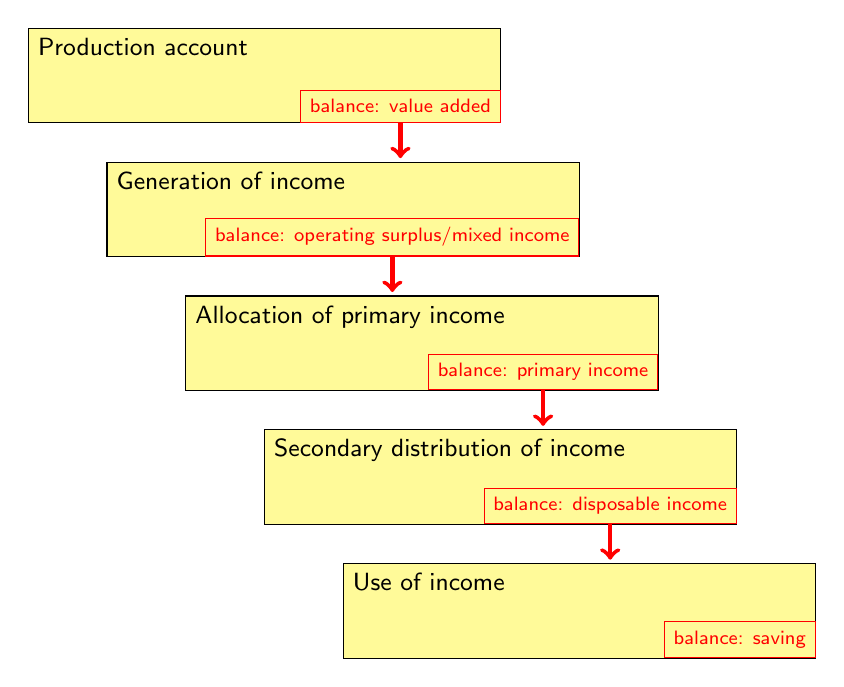
\begin{tikzpicture}
    \def\mystretch{1.7}
    \tikzset{
        myaccount/.style={
            draw,
            fill=yellow!40,
            font=\small\sffamily
        } 
    }
    \beameronly{\useasboundingbox (1,-1.7) rectangle (11,-9.7);}
    \foreach[count=\i, remember=\i as \prev (initially 0)] \myaccount/\mybalance in 
        {%
        Production account/value added,
        Generation of income/{operating surplus/mixed income},
        Allocation of primary income/primary income,
        Secondary distribution of income/disposable income,
        Use of income/saving%
        }
        {
            \ifstep{\i}{
                \draw[myaccount] (\i,-\mystretch*\i) 
                    node[below right] (A\i) {\myaccount}
                rectangle (6+\i,-\mystretch*\i-1.2)
                    node[above left,draw,red] (B\i) {\scriptsize balance: \mybalance}
                ;
            \ifnum\i>1
            \draw[->,red,ultra thick] (B\prev.south) -- ++(0,-0.45);
            \fi
            }
        }

\end{tikzpicture}
\end{document}